\documentclass{standalone}
\usepackage{tikz}

\begin{document}

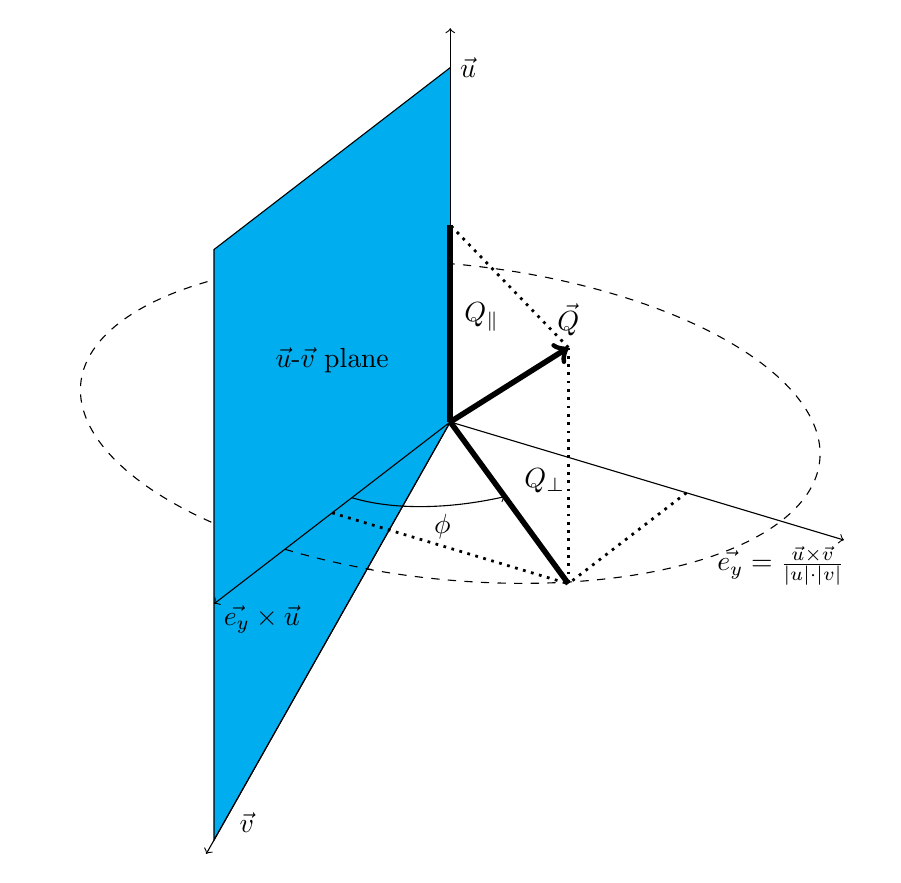
\begin{tikzpicture}[x={(-5mm,-3.85mm)},z={(0,1cm)},y={(1cm,-.3cm)}]

  \draw [,dashed] (0,0,0) ellipse (4.2 and 4.2) [below];	
  \draw [fill=cyan] (0,0,0)--(6,0,-3)--(6,0,4.5)--(0,0,4.5) node [above, xshift=-1.5cm,yshift=-4cm] {$\vec{u}$-$\vec{v}$ plane};
  \draw [,dashed] (4.2,0,0) arc [start angle=0,end angle=15,x radius=4,y radius=4.];	  
  
  \draw [line width=2pt] (0,0,0)--(0,0,2.5) node [above,xshift=0.4cm,yshift=-1.5cm] {$Q_{\|}$};
  \draw [->] (0,0) -- (6.2,0,-3.1) node [right,xshift=0.3cm,yshift=.4cm] {$\vec{v}$};
  \draw [->] (0,0) -- (0,5,0) node [above,xshift=-0.8cm,yshift=-0.7cm] {$\vec{e_y} = \frac{\vec{u} \times \vec{v}}{|u|\cdot |v|}$};
  \draw [->] (0,0) -- (0,0,5) node [right,yshift=-0.5cm] {$\vec{u}$};

  \draw [->] (0,0) -- (6,0,0) node [right,xshift=-0.0cm,yshift=-0.2cm] {$\vec{e_y} \times \vec{u}$};

  \draw [line width=1pt,dotted] (3,3,3) -- (0,0,2.5);=
  
  \draw [line width=1pt,dotted] (0,3,0)  -- (3,3,0);
  \draw [line width=1pt,dotted] (3,0,0) -- (3,3,0);  
=
  \draw [line width=2pt, ->] (0,0,0) -- (3,3,3) node [above] {$\vec{Q}$};
  \draw [line width=1pt,dotted] (3,3,3) -- (3,3,0);
  \draw [line width=2pt] (0,0,0) -- (3,3,0) node [above,xshift=-0.3cm,yshift=1cm] {$Q_{\perp}$};

  \draw [->] (2.5,0,0) arc [start angle=0,end angle=44,x radius=4,y radius=2] node [below,xshift=-0.8cm,yshift=-0.1cm] {$\phi$};
  

\end{tikzpicture}

\end{document}
